\documentclass[professionalfonts,aspectratio=169]{beamer}

\usetheme{Madrid}
\usecolortheme{seagull}
\setbeamertemplate{navigation symbols}{}
\setbeamerfont{footnote}{size=\tiny}
\setbeamersize{text margin left=1.2em,text margin right=1.2em}

\usepackage{amsmath,amssymb,mathtools}
\usepackage{graphicx}
\usepackage{booktabs}
\usepackage{tikz}
\usepackage{array}
\usepackage{adjustbox}

\definecolor{mainblue}{RGB}{23,79,132}
\definecolor{accentorange}{RGB}{233,130,20}
\setbeamercolor{structure}{fg=mainblue}
\setbeamercolor{title}{fg=white,bg=mainblue}
\setbeamercolor{frametitle}{fg=mainblue}
\setbeamerfont{frametitle}{series=\bfseries,size=\Large}
\setbeamerfont{subtitle}{size=\large}
\setbeamerfont{normal text}{size=\small}
\setbeamertemplate{itemize item}{\color{accentorange}$\blacktriangleright$}
\setbeamertemplate{itemize subitem}{\color{mainblue}$\bullet$}

\newcommand{\headlinebar}{\tikz{\fill[mainblue!80] (0,0) rectangle (0.16,0.16);}\,}

\addtobeamertemplate{frametitle}{}{\vspace{-0.7ex}\rule{\linewidth}{0.6pt}\vspace{-0.3ex}}

\title{H\&E $\rightarrow$ ORION Virtual Multiplexing}
\subtitle{Briefing}
\author{RA Biomed ML Team}
\date{5 November 2025}

\begin{document}

\begin{frame}[plain]
  \titlepage
\end{frame}

\begin{frame}{Clinical Motivation}
  \begin{itemize}
    \item Accelerate multiplex immunofluorescence (Orion, 20 channels) by predicting from routine H\&E.
    \item Reduce wet-lab turnaround for macrophage-rich TA118 cohort; prioritise atypical regions.
    \item Provide spatial biomarker estimates to support therapy stratification and rapid QC.
  \end{itemize}
\end{frame}

\begin{frame}{Workflow Overview}
  \begin{columns}[T]
    \begin{column}{0.48\textwidth}
      \begin{itemize}
        \item VALIS rigid \& non-rigid registration (Bio-Formats reader).
        \item Tissue segmentation via Laplacian $+$ Otsu, morphological cleanup.
        \item Crop aligned slides into 2048$\times$2048 cores centred on tissue.
      \end{itemize}
    \end{column}
    \begin{column}{0.48\textwidth}
      \begin{itemize}
        \item Global quantile scaler (train-set only) for Orion intensities.
        \item Stratified sampling to favour rare/speckled markers.
        \item Distributed (DDP) training with mixed precision and channel-aware losses.
      \end{itemize}
    \end{column}
  \end{columns}
\end{frame}

\begin{frame}{Dataset Snapshot}
  \begin{itemize}
    \item 319 paired cores exported as float32 NPY (`core\_***`).
    \item Orion cube consistently 20 channels; H\&E normalised to [0,1].
    \item Train/val split: deterministic stratification (seeded shuffle).
    \item Quantile scaler persisted to `orion\_scaler.json` and broadcast to all ranks.
  \end{itemize}
\end{frame}

\begin{frame}{Marker Panel Highlights}
  \begin{itemize}
    \item Macrophage subsets: SPP1, FOLR2, NLRP3, LYVE1, IL4I1.
    \item Immune context: HLA-DR (DC), CD3\,$\varepsilon$, CD8$\alpha$, FOXP3, CD15.
    \item Tumor/stroma: Pan-CK, SMA, FAP, GFPT2.
    \item Supports spatial mapping of immune suppression, fibrosis, vascular niches.
  \end{itemize}
\end{frame}

\begin{frame}{Quantitative Insights}
  \begin{columns}[T]
    \begin{column}{0.48\textwidth}
      \begin{itemize}
        \item Coverage at threshold 0.08 spans $\sim$12\% (ch00) to $<0.01\%$ (ch05/ch16).
        \item Mean intensities highly skewed; motivates per-channel scaling and sampling.
        \item Speckle-heavy markers (ch02, ch13, ch11) require regularisation.
      \end{itemize}
    \end{column}
    \begin{column}{0.48\textwidth}
      \includegraphics[width=\textwidth,height=0.42\textheight,keepaspectratio]{../output/data_summary_nov4/plots/channel_coverage.png}\\[4pt]
      \includegraphics[width=\textwidth,height=0.42\textheight,keepaspectratio]{../output/data_summary_nov4/plots/channel_mean_intensity.png}
    \end{column}
  \end{columns}
\end{frame}

\begin{frame}{Pipeline Diagram}
  \centering
  \fbox{\parbox{0.85\textwidth}{\centering INSERT PIPELINE SCHEMATIC\\(Registration $\rightarrow$ Tissue detection $\rightarrow$ Core export $\rightarrow$ Training)}}
\end{frame}

\begin{frame}{Training Configuration}
  \begin{itemize}
    \item Input patches: 224$\times$224, augmentations (flip, rotate, color jitter, resize).
    \item Oversample positives: $p=0.65$ with channel-aware probabilities from coverage stats.
    \item Optimiser: AdamW (lr $3\times 10^{-4}$), cosine decay $\pm$ warmup, grad clip 1.0.
    \item Loss blend: center-weighted MSE + coverage penalty + MS-SSIM (optional) + TV + presence head.
    \item Multi-GPU torchrun (DDP) with AMP; best checkpoints tracked via val loss.
  \end{itemize}
\end{frame}

\begin{frame}{Quantile Scaling \& Log Transform}
  \begin{columns}[T]
    \begin{column}{0.55\textwidth}
      \small
      For Orion intensity $x_{c}(u,v)$ in channel $c$:
      \begin{align*}
        \tilde{x}_{c}(u,v) &= \frac{x_{c}(u,v) - q_{c}^{\text{low}}}{q_{c}^{\text{high}} - q_{c}^{\text{low}} + 10^{-6}} \\
        z_{c}(u,v) &= \log\big(1 + \max(\tilde{x}_{c}(u,v), 0)\big)
      \end{align*}
      \begin{itemize}
        \item $q_{c}^{\text{low}}, q_{c}^{\text{high}}$: global train-set quantiles (1\%, 99.5\%).
        \item Stabilises dynamic range; prevents bright outliers from dominating gradients.
        \item Log transform makes low-intensity “dot” markers resolvable and aligns with Poisson-like noise.
      \end{itemize}
    \end{column}
    \begin{column}{0.42\textwidth}
      \footnotesize
      \begin{block}{Why pathologists care}
        \begin{itemize}
          \item Preserves relative marker ordering across cores.
          \item Enables consistent back-transformation for ORION review ($\exp(z)-1$).
          \item Avoids over-saturation of stromal-rich or hemorrhagic regions.
        \end{itemize}
      \end{block}
      \vspace{0.5em}
      \includegraphics[width=\textwidth,height=0.42\textheight,keepaspectratio]{../output/data_summary_nov4/plots/channel_speckle_bar.png}
    \end{column}
  \end{columns}
\end{frame}

\begin{frame}{Swin-UNet Architecture}
  \begin{columns}[T]
    \begin{column}{0.52\textwidth}
      \begin{itemize}
        \item Encoder: `swin\_tiny\_patch4\_window7\_224` (windowed self-attention).
        \item Feature pyramid with 1$\times$1 lateral projections to 192 channels.
        \item Bilinear upsample + skip summation; decoder halves width before Softplus output.
        \item Excels at long-range morphology patterns, robust to sparse signals.
      \end{itemize}
    \end{column}
    \begin{column}{0.44\textwidth}
      \fbox{\parbox{\textwidth}{\centering INSERT SWIN-UNET DIAGRAM}}
    \end{column}
  \end{columns}
\end{frame}

\begin{frame}{ConvNeXt-UNet Variant}
  \begin{columns}[T]
    \begin{column}{0.52\textwidth}
      \begin{itemize}
        \item Encoder: `convnext\_tiny` (hierarchical depthwise conv blocks).
        \item Shares decoder topology; emphasises local texture cues.
        \item Faster convergence on abundant markers; more variance on speckled channels.
        \item Lower computational footprint, candidate for edge deployment.
      \end{itemize}
    \end{column}
    \begin{column}{0.44\textwidth}
      \fbox{\parbox{\textwidth}{\centering INSERT CONVNEXT-UNET DIAGRAM}}
    \end{column}
  \end{columns}
\end{frame}

\begin{frame}{Loss Design and Sampling}
  \small
  \begin{columns}[T]
    \begin{column}{0.51\textwidth}
      \textbf{Composite loss}
      \begin{align*}
        \mathcal{L} &= \lambda_{\text{mse}}\,\mathcal{L}_{\text{center}} + \lambda_{\text{cov}}\,\mathcal{L}_{\text{cov}} + \lambda_{\text{SSIM}}\,\mathcal{L}_{\text{MS-SSIM}}\\
                   &\quad + \lambda_{\text{TV}}\,\mathcal{L}_{\text{TV}} + \lambda_{\text{pres}}\,\mathcal{L}_{\text{presence}}
      \end{align*}
      \vspace{-0.5em}
      \begin{align*}
        \mathcal{L}_{\text{center}} &= \frac{1}{|\Omega|} \sum_{(u,v) \in \Omega} w_{c}(u,v) \big(y_{c}(u,v) - \hat{y}_{c}(u,v)\big)^{2}\\
        w_{c}(u,v) &= 1 + \gamma \mathbb{1}\{\hat{y}_{c}(u,v) > \tau\}
      \end{align*}
      \begin{itemize}
        \item $\Omega$: 12$\times$12 central window; emphasises diagnostically annotated zone.
        \item $\gamma=3$ boosts pixels above log-threshold $\tau=0.10$—stops “washing out” rare spots.
        \item Channel weight map multiplies $w_{c}$ using inverse coverage statistics (caps pathology noise).
      \end{itemize}
    \end{column}
    \begin{column}{0.46\textwidth}
      \textbf{Auxiliary terms}
      \begin{align*}
        \mathcal{L}_{\text{cov}} &= \left\| \bar{y}_{c} - \bar{\hat{y}}_{c} \right\|_{1} \quad (\text{per-channel mean matching})\\
        \mathcal{L}_{\text{MS-SSIM}} &= 1 - \text{MS-SSIM}(y,\hat{y})\\
        \mathcal{L}_{\text{TV}} &= \|\nabla_{h} \hat{y}\|_{1} + \|\nabla_{v} \hat{y}\|_{1}\\
        \mathcal{L}_{\text{presence}} &= \text{BCEWithLogits}\big(\logit_{c}, \mathbb{1}\{\hat{y}_{c}^{\max} > \tau\}\big)
      \end{align*}
      \begin{itemize}
        \item $\bar{y}_{c}$: spatial average intensity—keeps global abundance realistic.
        \item TV discourages hallucinated speckle noise while preserving sharp edges.
        \item Presence head gives on/off probability per marker, aiding triage dashboards.
      \end{itemize}
    \end{column}
  \end{columns}
\end{frame}

\begin{frame}{Adaptive Sampling Strategy}
  \begin{columns}[T]
    \begin{column}{0.53\textwidth}
      \small
      \textbf{Per-channel probability}
      \begin{align*}
        p_{c} &\propto \left(\frac{1}{\text{coverage}_{c} + 10^{-4}}\right)^{\alpha} (\text{mean}_{c} + 10^{-4})\\
        \alpha &= 1.0,\; p_{c} = \frac{p_{c}}{\sum_{k} p_{k}}
      \end{align*}
      \begin{itemize}
        \item Encourages sampling of channels with scarce positive pixels.
        \item Speckle-heavy top-$k$ (2, 13, 11, 0) double resample budget to catch rare dots.
      \end{itemize}
      \textbf{Patch acceptance}
      \begin{align*}
        \text{accept if} \;&\exists c\in \{c^{*},\text{all}\}: \frac{|\{(u,v): y_{c}(u,v) > \tau\}|}{ps^{2}} > \epsilon_{c}
      \end{align*}
      with $\epsilon_{c}=0.002$ for targeted channel, $0.005$ otherwise.
    \end{column}
    \begin{column}{0.44\textwidth}
      \footnotesize
      \begin{block}{Clinical rationale}
        \begin{itemize}
          \item Guarantees each mini-batch contains macrophage-rich examples.
          \item Aligns model focus with markers flagged by pathologists for TA118.
          \item Sampling metadata ($c^{*}$) logged for auditability and error analysis.
        \end{itemize}
      \end{block}
      \vspace{0.6em}
      \includegraphics[width=\textwidth,height=0.4\textheight,keepaspectratio]{../output/data_summary_nov4/plots/channel_speckle_vs_coverage.png}
    \end{column}
  \end{columns}
\end{frame}

\begin{frame}{Training Metrics}
  \centering
  \fbox{\parbox{0.85\textwidth}{\centering INSERT TRAIN/VAL LOSS CURVES\\(e.g., metrics from `runs_*` once exported)}}
\end{frame}

\begin{frame}{Qualitative Data QC}
  \begin{columns}[T]
    \begin{column}{0.48\textwidth}
      \includegraphics[width=\textwidth,height=0.45\textheight,keepaspectratio]{../output/visualize_nov4/core_001_he.png}\\[4pt]
      \includegraphics[width=\textwidth,height=0.45\textheight,keepaspectratio]{../output/visualize_nov4/core_007_he.png}
    \end{column}
    \begin{column}{0.48\textwidth}
      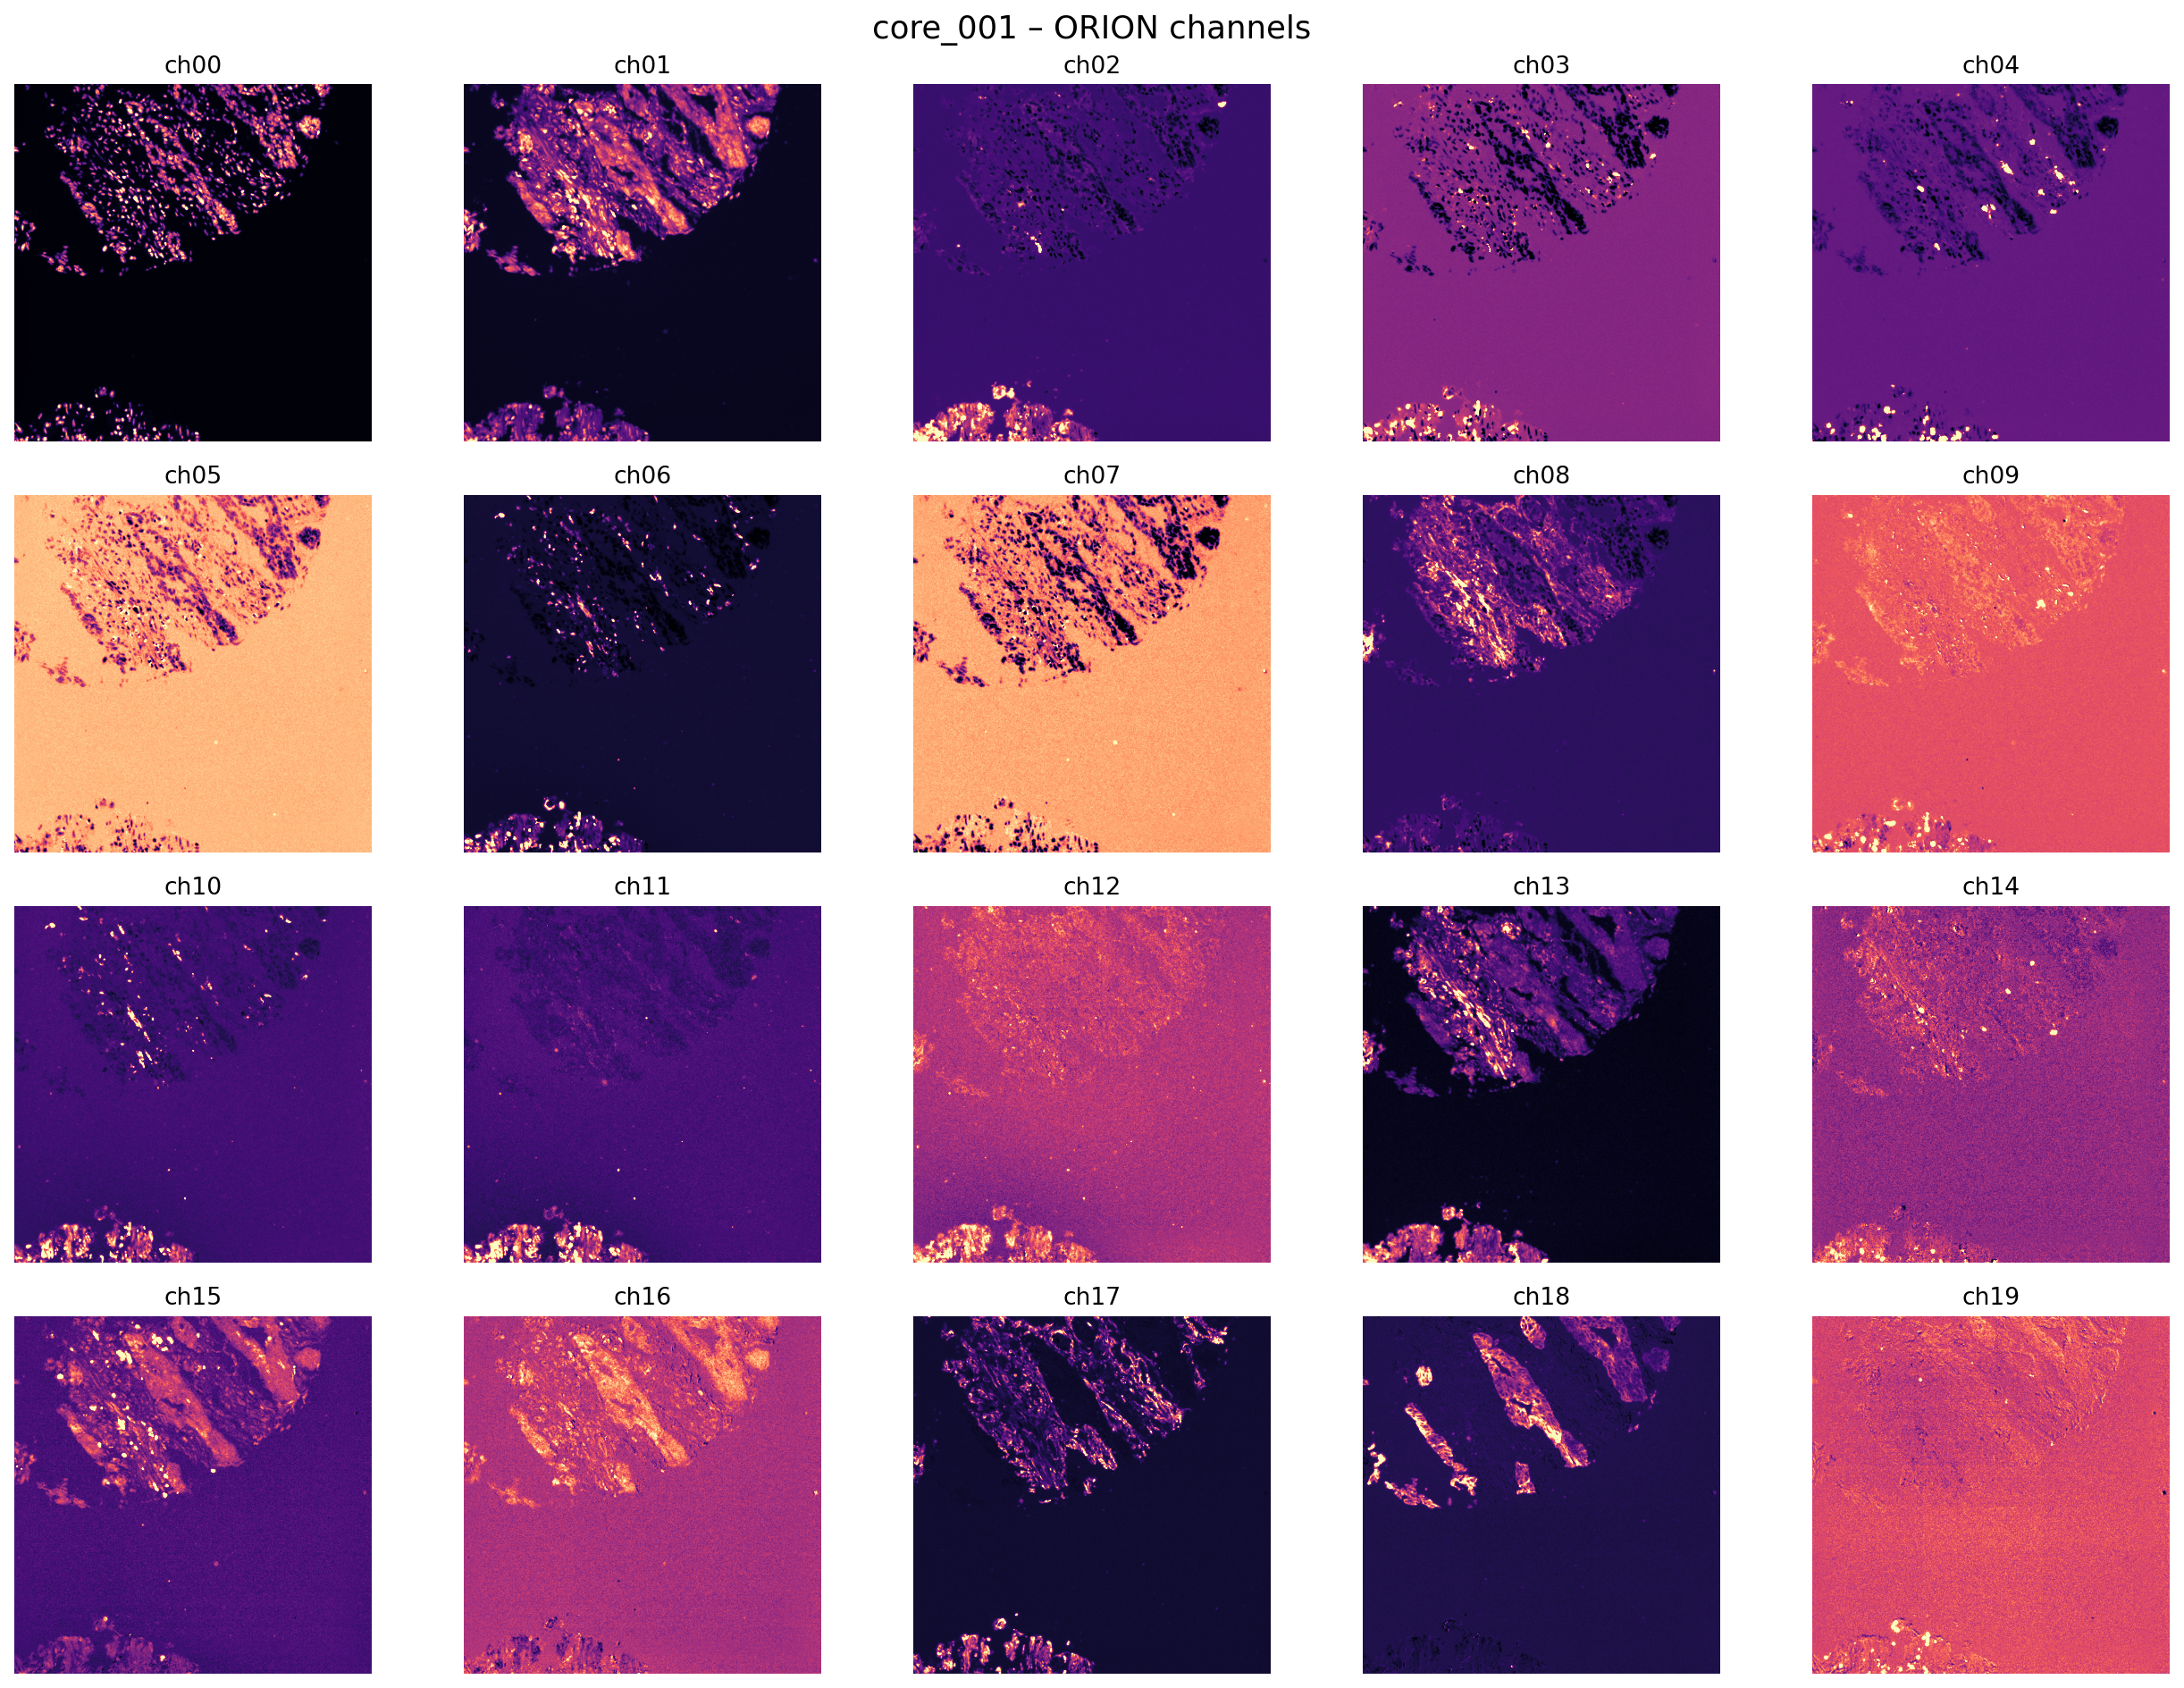
\includegraphics[width=\textwidth,height=0.45\textheight,keepaspectratio]{../output/visualize_nov4/core_001_orion_channels.png}\\[4pt]
      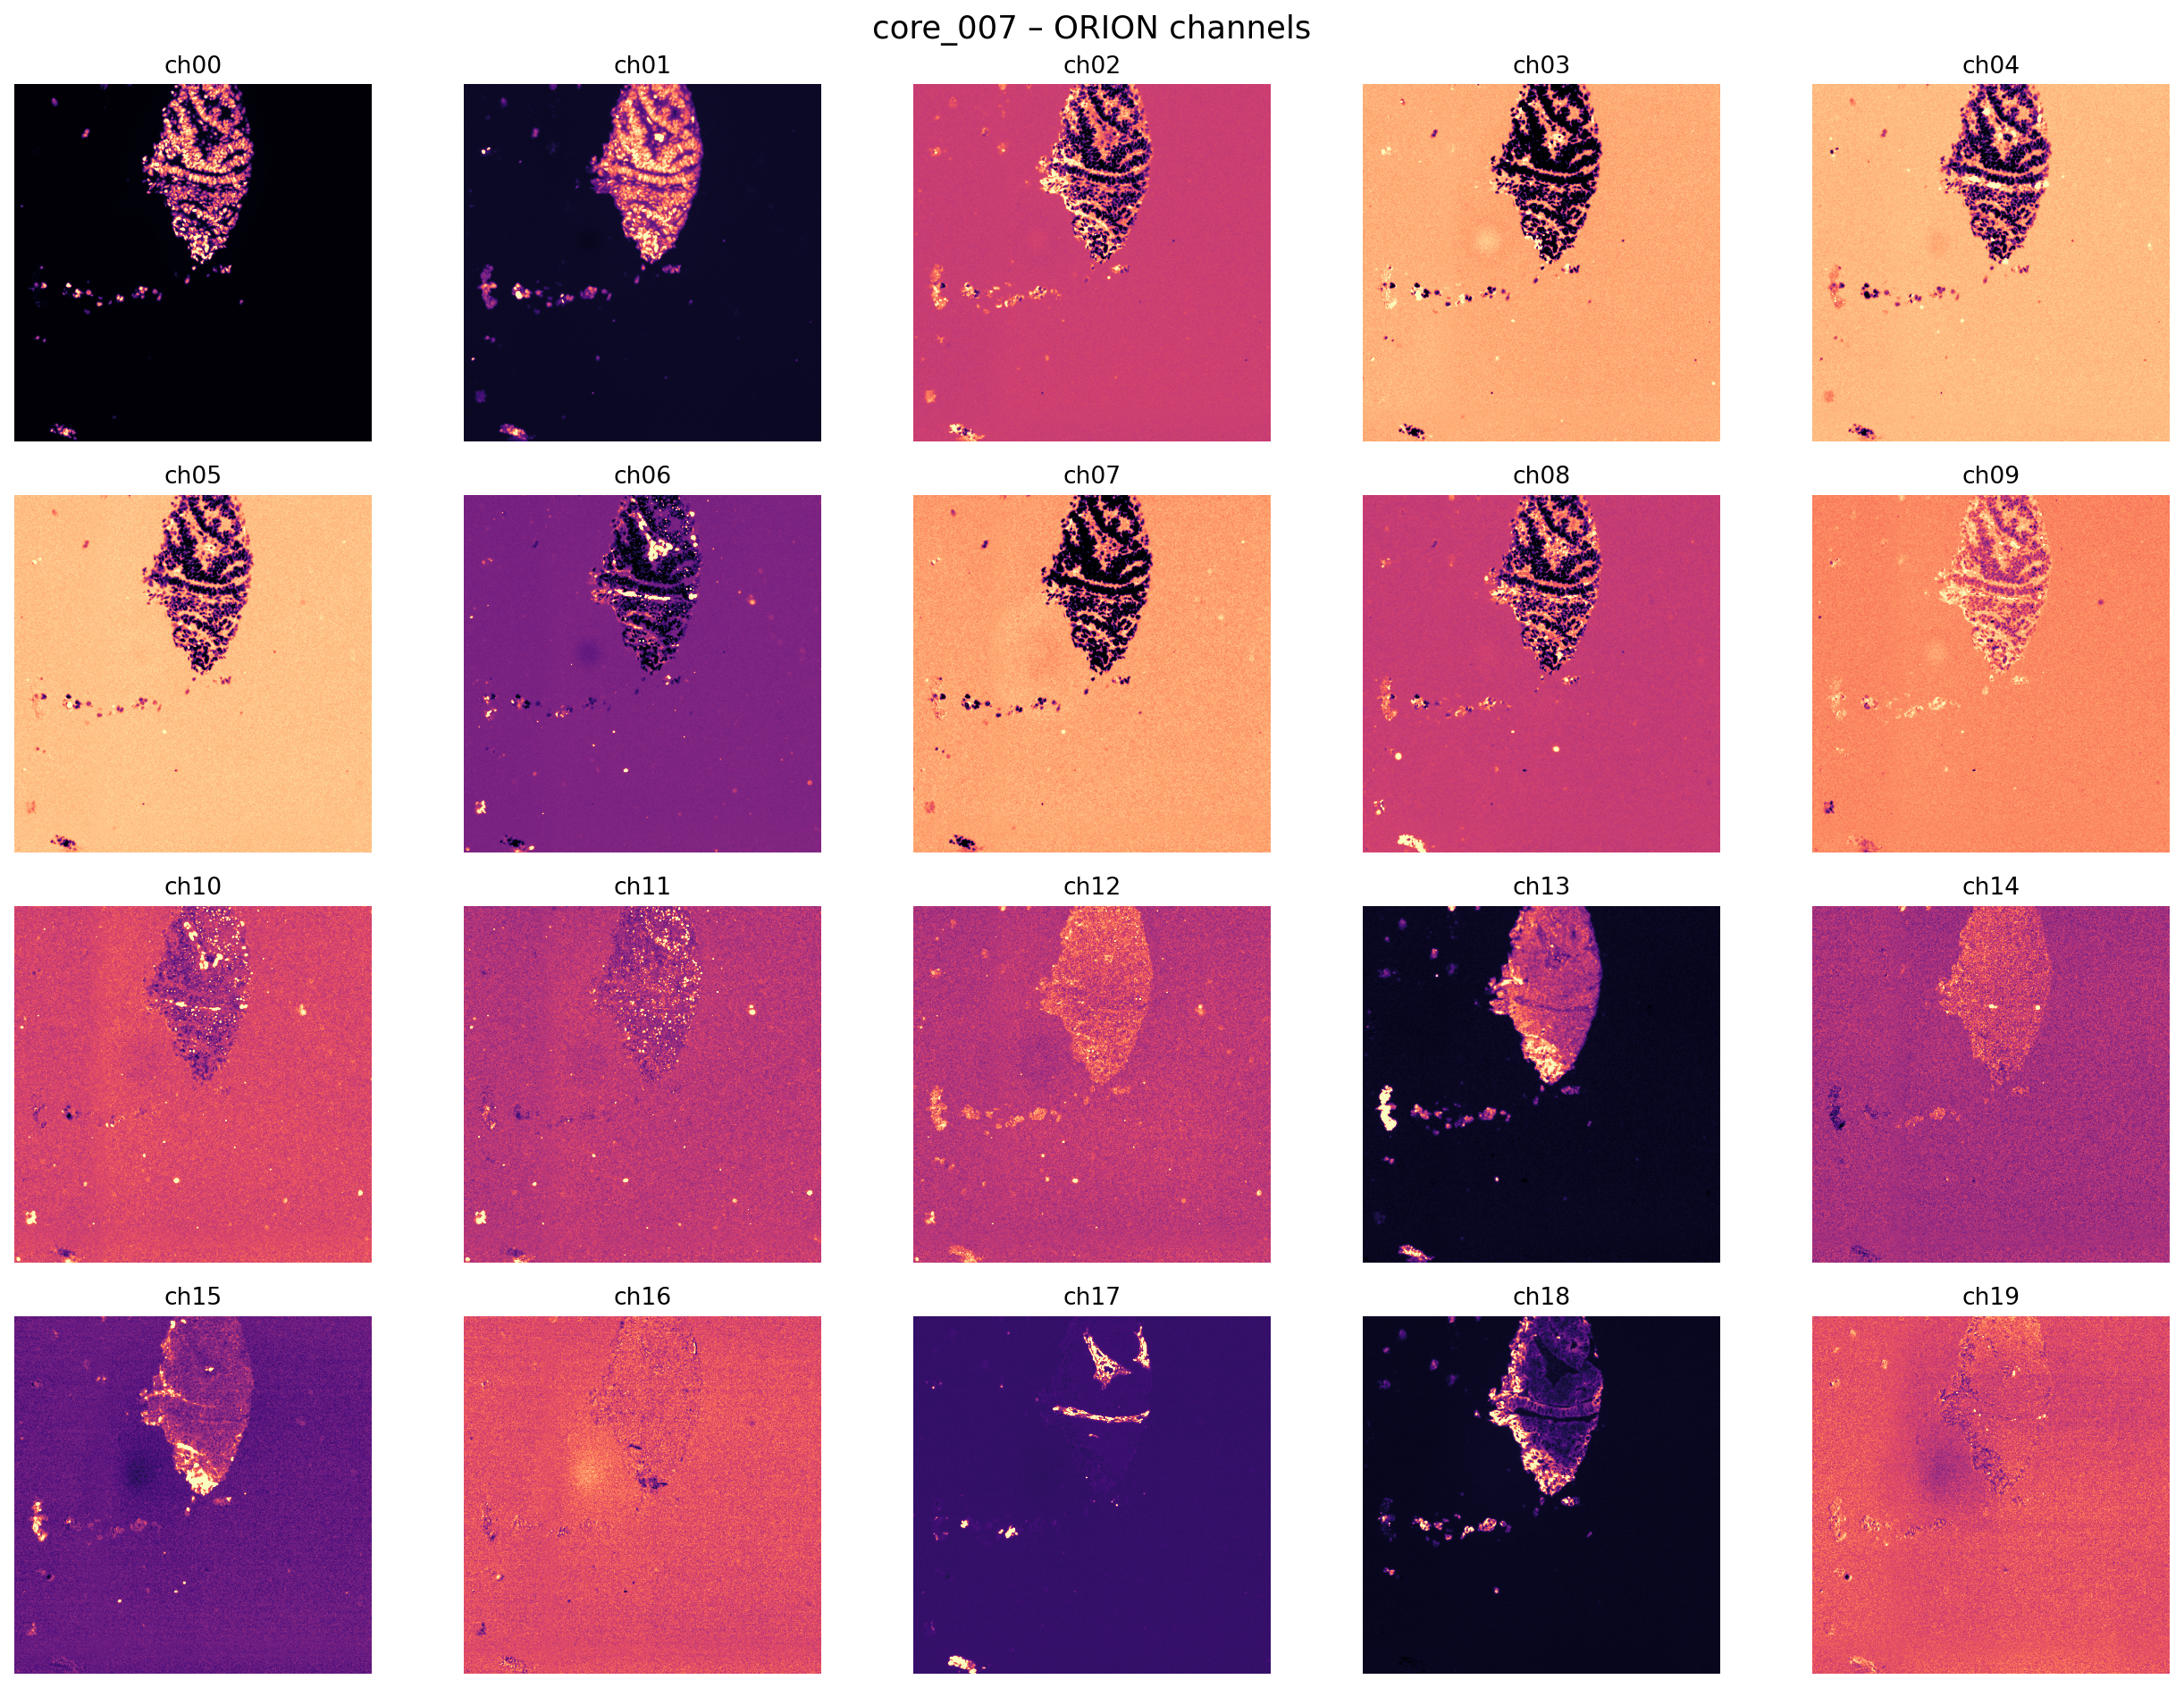
\includegraphics[width=\textwidth,height=0.45\textheight,keepaspectratio]{../output/visualize_nov4/core_007_orion_channels.png}
    \end{column}
  \end{columns}
\end{frame}

\begin{frame}{Extended QC Gallery}
  \begin{columns}[T]
    \begin{column}{0.48\textwidth}
      \includegraphics[width=\textwidth,height=0.45\textheight,keepaspectratio]{../output/visualize_nov4/core_073_he.png}\\[4pt]
      \includegraphics[width=\textwidth,height=0.45\textheight,keepaspectratio]{../output/visualize_nov4/core_272_he.png}
    \end{column}
    \begin{column}{0.48\textwidth}
      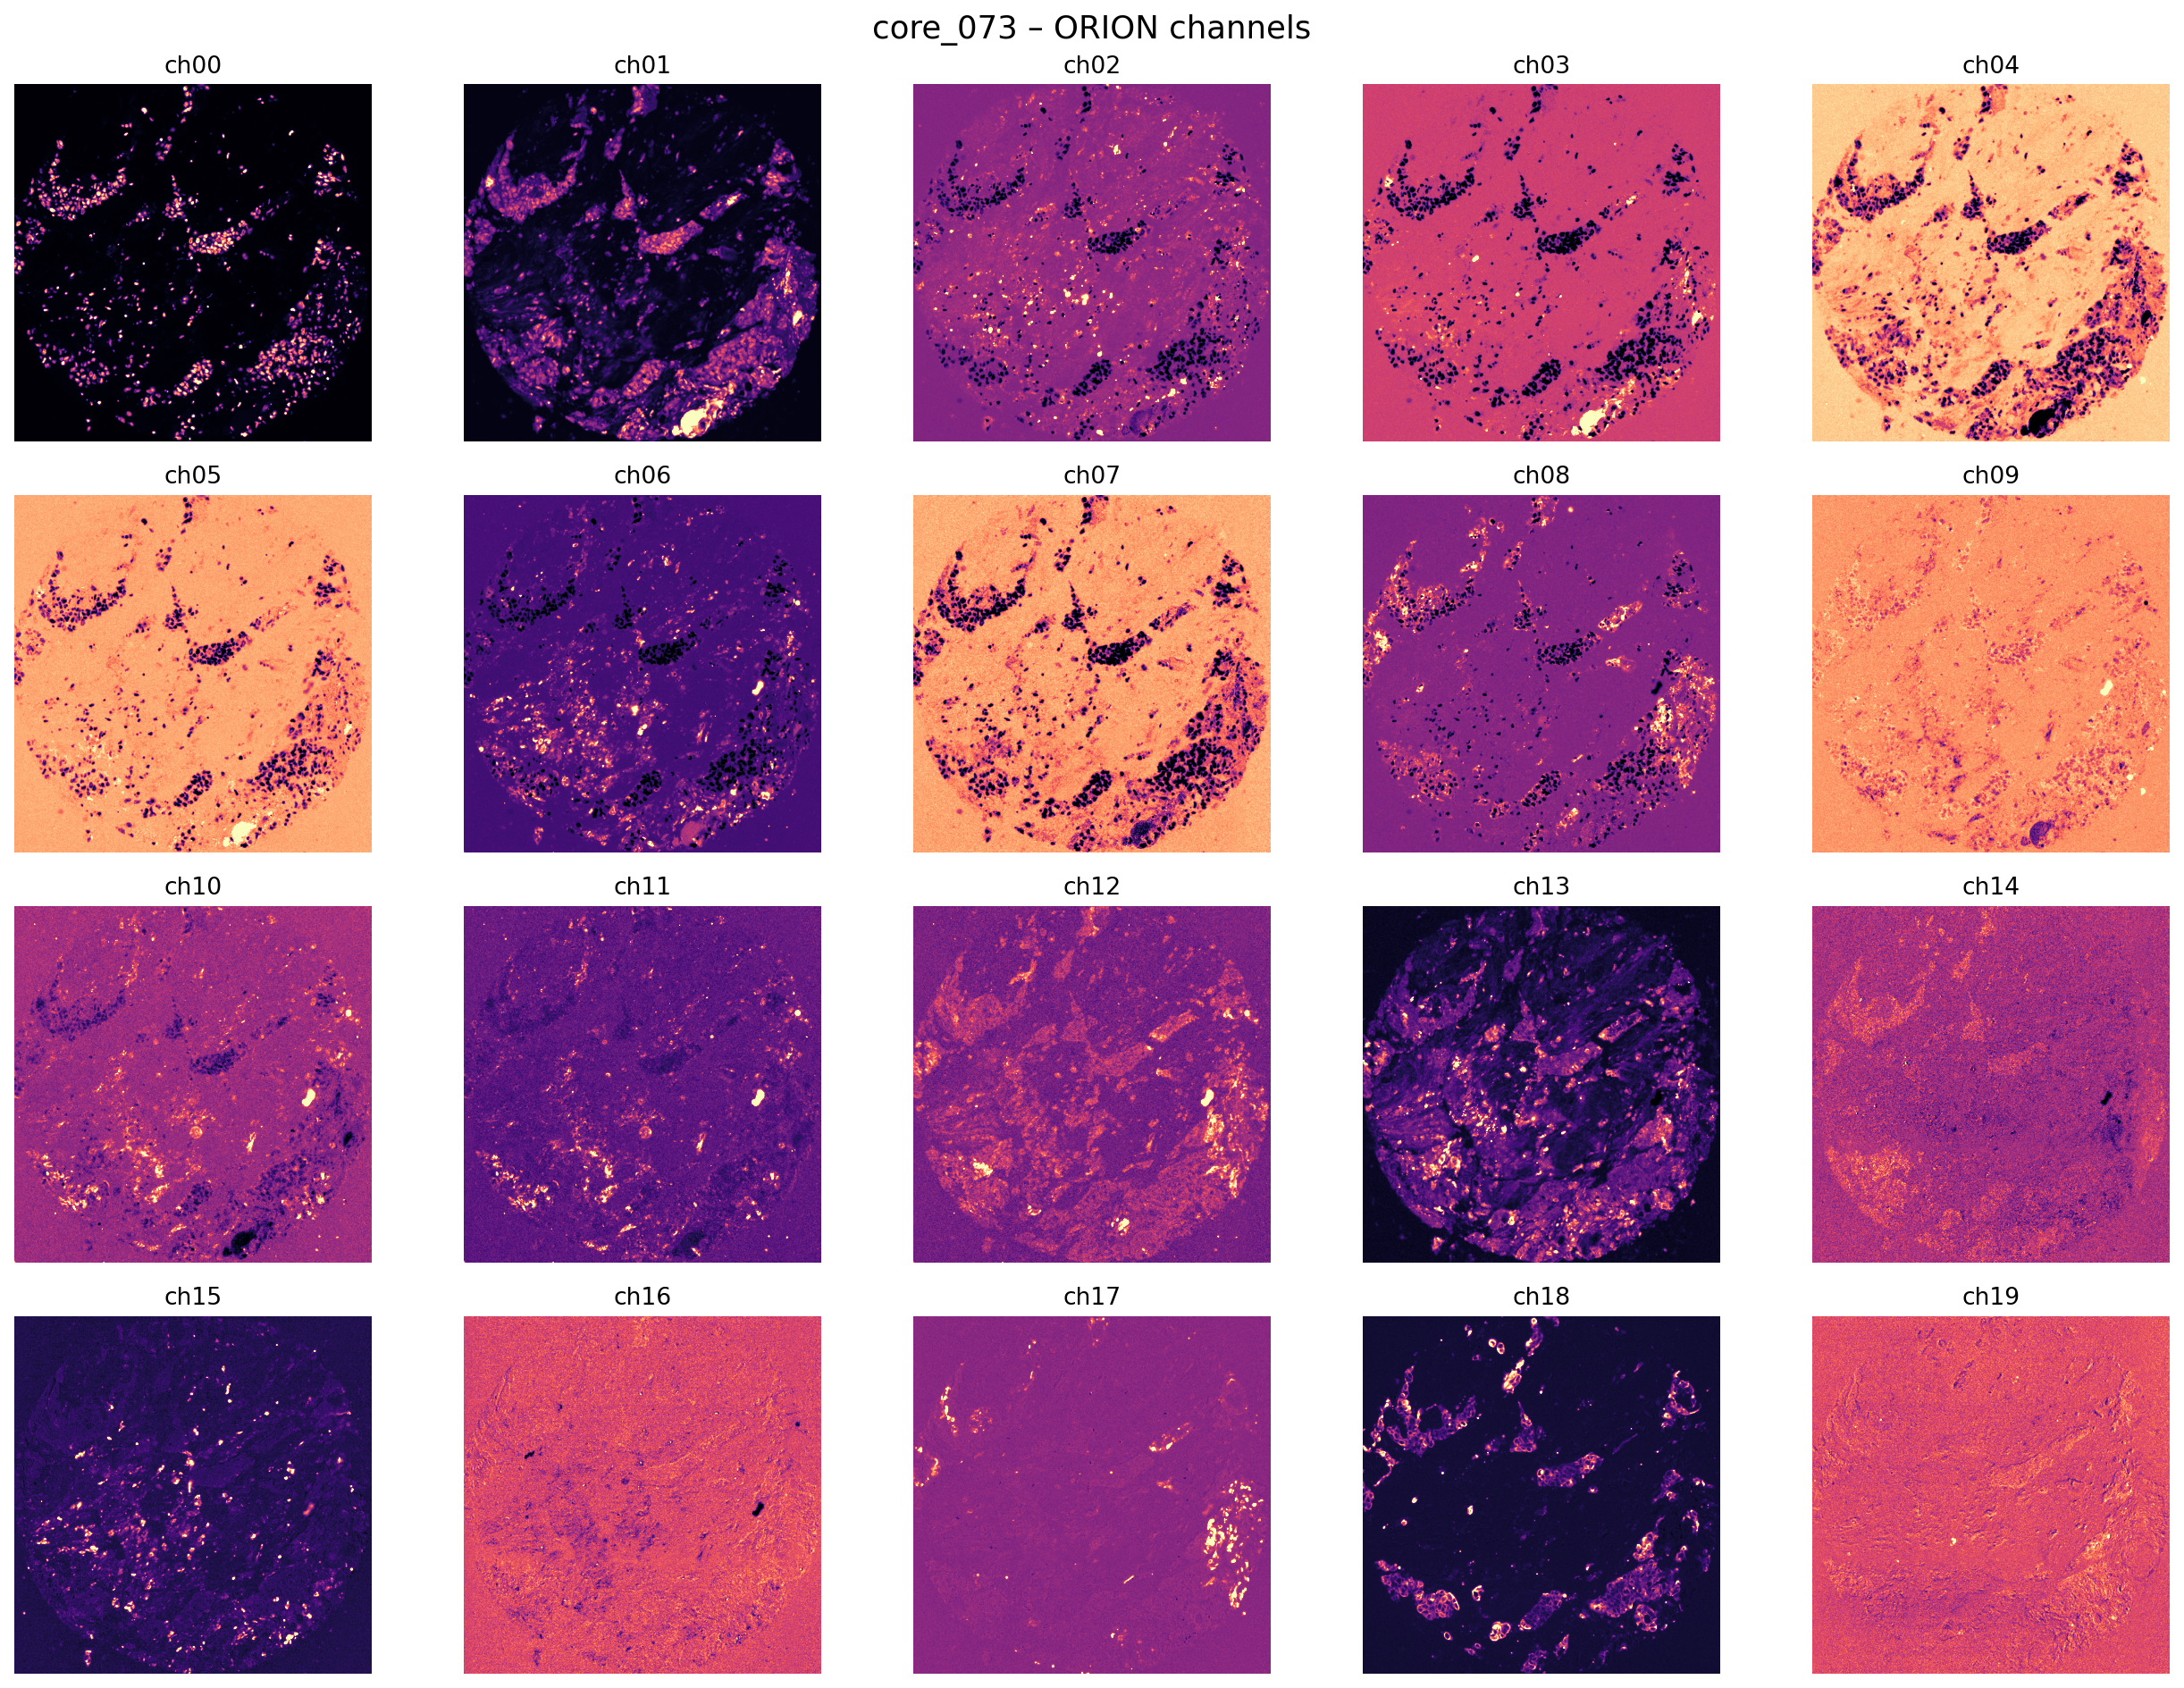
\includegraphics[width=\textwidth,height=0.45\textheight,keepaspectratio]{../output/visualize_nov4/core_073_orion_channels.png}\\[4pt]
      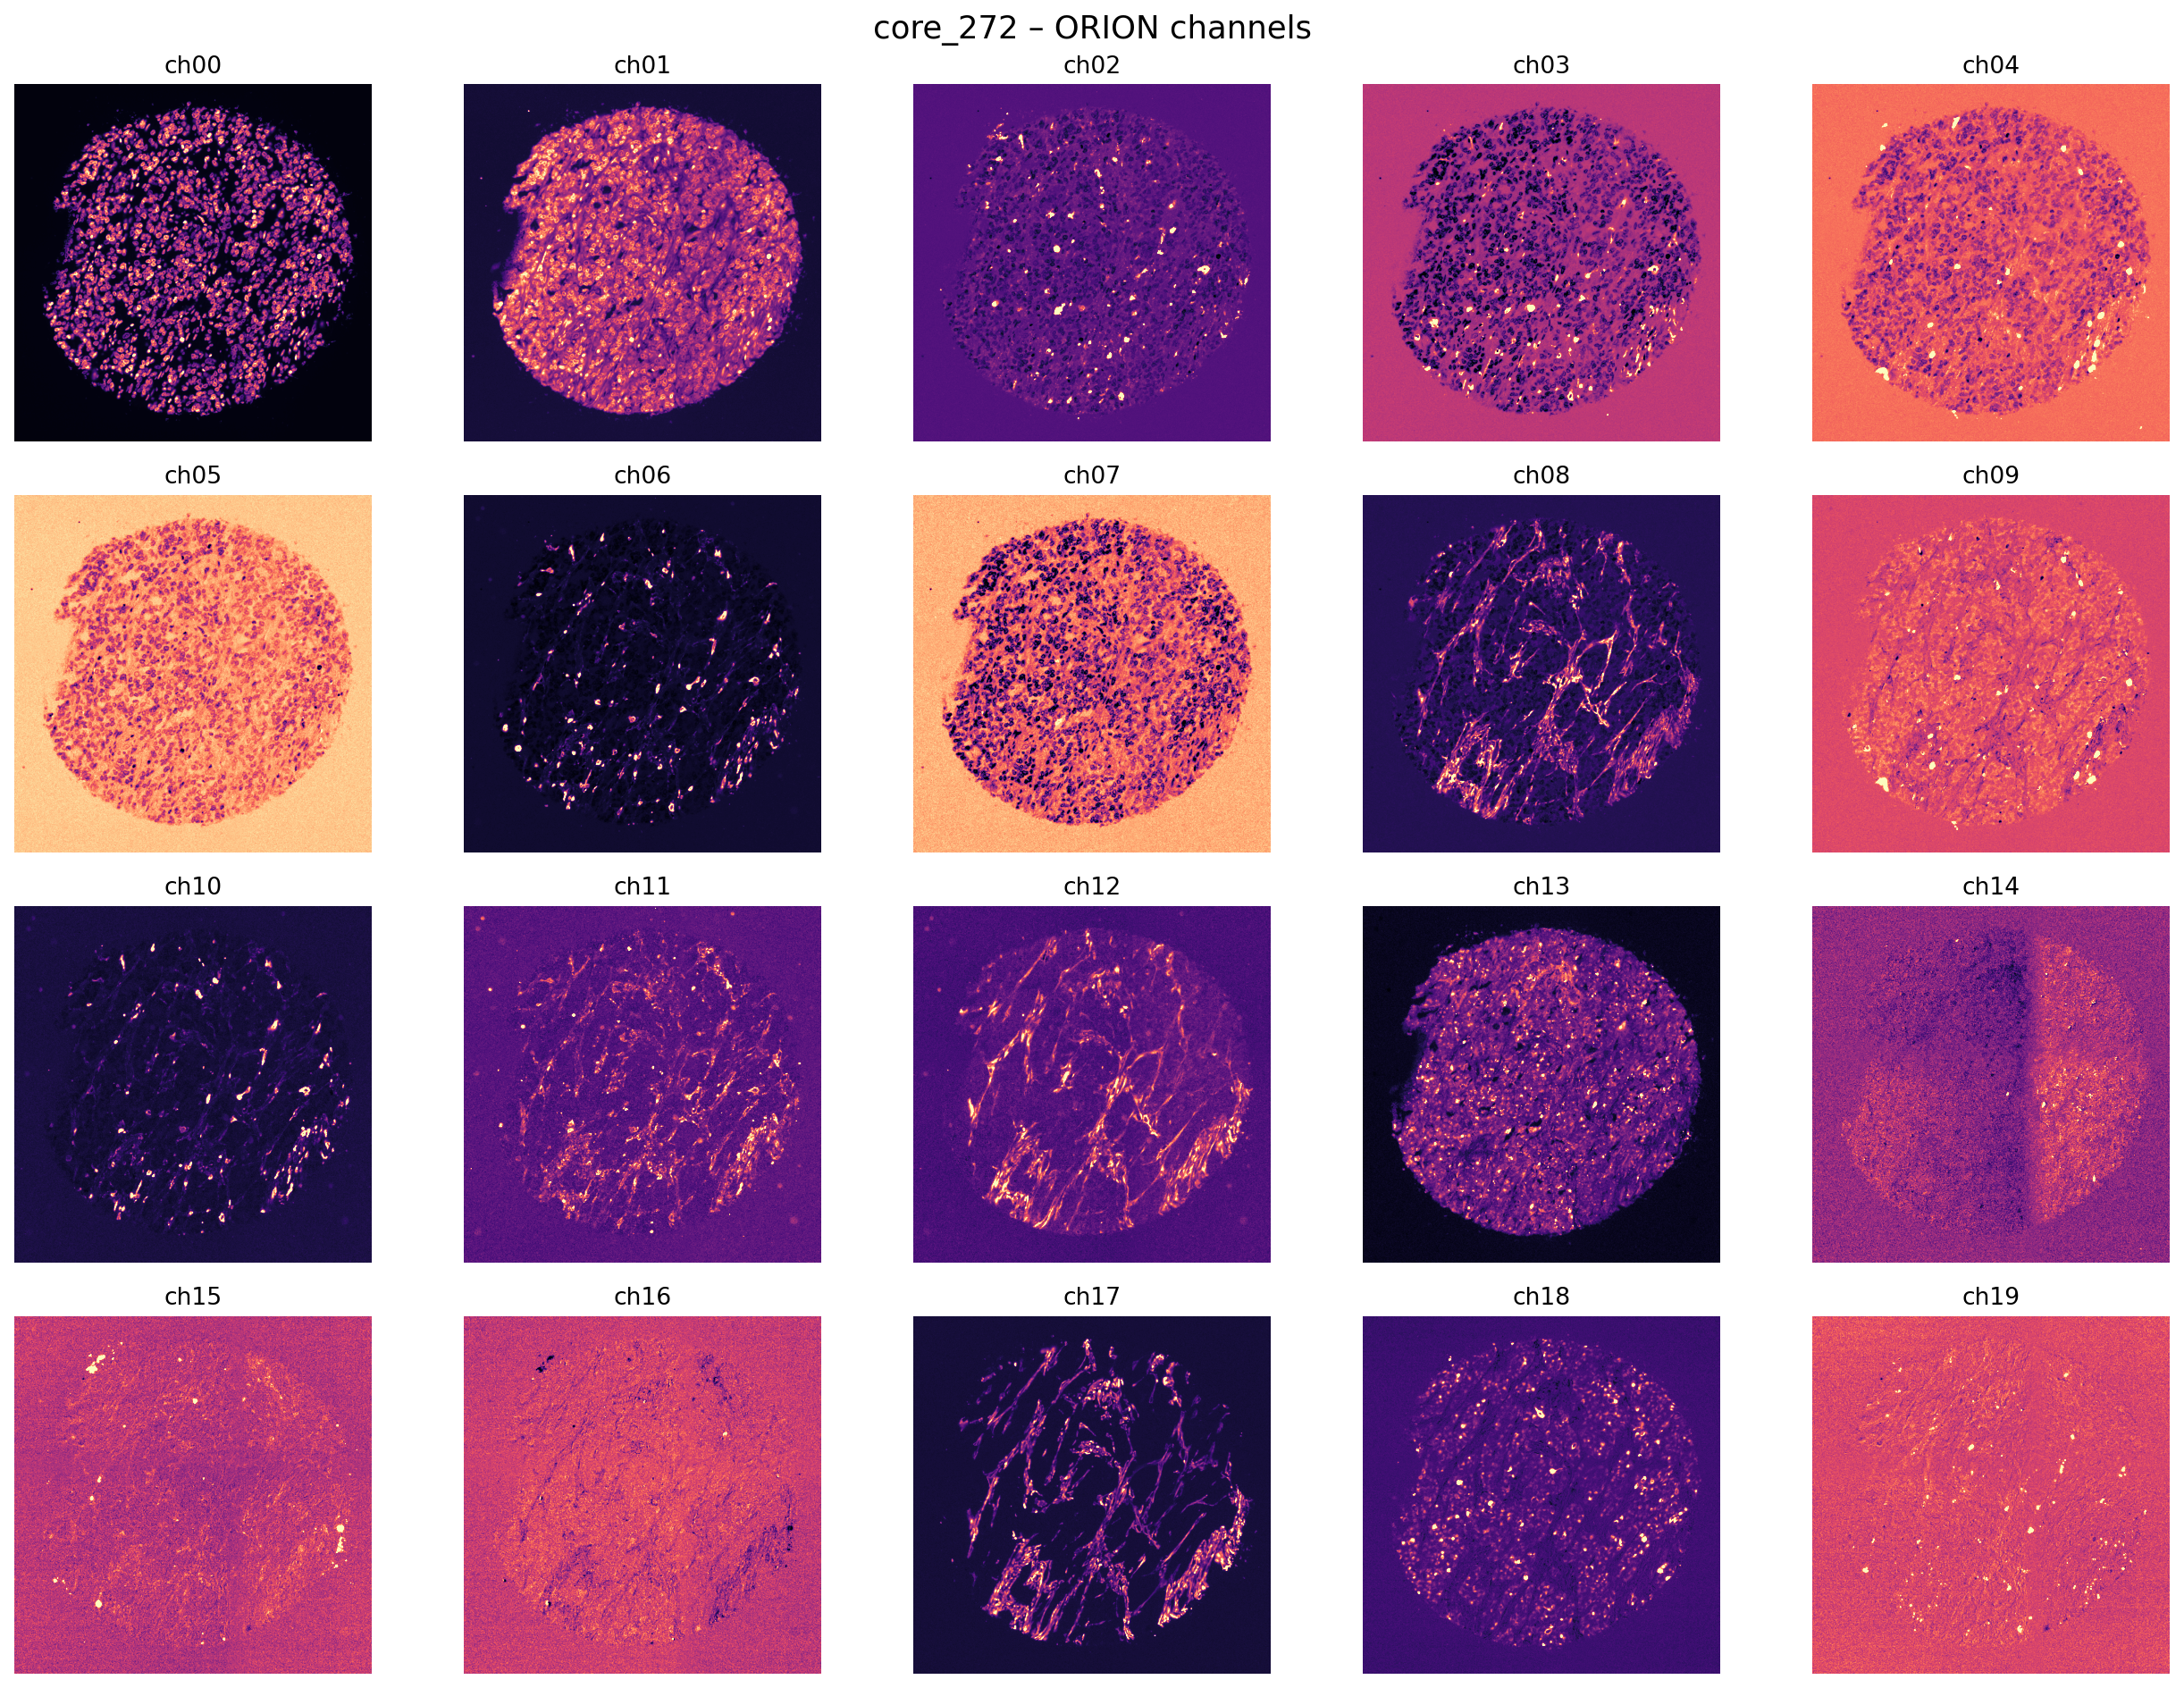
\includegraphics[width=\textwidth,height=0.45\textheight,keepaspectratio]{../output/visualize_nov4/core_272_orion_channels.png}
    \end{column}
  \end{columns}
\end{frame}

\begin{frame}{Model vs Ground Truth Placeholders}
  \begin{columns}[T]
    \begin{column}{0.48\textwidth}
      \fbox{\parbox{\textwidth}{\centering INSERT SWIN-UNET vs GT (core\_001)\\per-channel montage}}
    \end{column}
    \begin{column}{0.48\textwidth}
      \fbox{\parbox{\textwidth}{\centering INSERT CONVNEXT vs GT (core\_001)\\per-channel montage}}
    \end{column}
  \end{columns}
  \vspace{1em}
  \centering
  \fbox{\parbox{0.85\textwidth}{\centering INSERT CHANNEL TRIPTYCH (FOLR2 / CD163 / SPP1)}}
\end{frame}

\begin{frame}{Comparative Observations}
  \begin{itemize}
    \item Swin-UNet maintains morphology on sparse macrophage markers; reduced halo artefacts.
    \item ConvNeXt-UNet sharper on abundant epithelial markers (Pan-CK, SMA) but noisier on low coverage.
    \item Channel-aware sampling benefits both; evaluate cross-site generalisation in next phase.
    \item Future: ensemble or knowledge distillation to balance accuracy vs efficiency.
  \end{itemize}
\end{frame}

\begin{frame}{Novelty vs Literature}
  \begin{itemize}
    \item Full 20-channel Orion prediction with global quantile scaling and speckle-aware sampling.
    \item Presence-aware auxiliary head uncommon in prior H\&E $\rightarrow$ IF translation studies.
    \item End-to-end pipeline: registration, QC, DDP training for large cohorts.
    \item Extends beyond prior single-marker virtual staining and GAN-based approaches.
  \end{itemize}
\end{frame}

\begin{frame}{Related Work}
  \begin{itemize}
    \item Rivenson et al., \emph{PNAS} 2019: Virtual staining of auto-fluorescence (single channel).
    \item Fu et al., \emph{Nat. Biomed. Eng.} 2020: Hyperspectral marker imputation without channel-aware sampling.
    \item Lu et al., \emph{Med. Image Anal.} 2022: GAN-based H\&E $\rightarrow$ IF translation, limited scaling.
  \end{itemize}
  \vspace{0.5em}
  \centering
  \fbox{\parbox{0.85\textwidth}{\centering ADDITIONAL REFERENCES / DOI LINKS AS NEEDED}}
\end{frame}

\begin{frame}{Pathologist-Focused Takeaways}
  \begin{itemize}
    \item Rapid in silico multiplexing to prioritise cores for lab validation.
    \item Channel coverage maps and presence logits offer interpretability hooks.
    \item Feedback requested: critical markers, acceptable error ranges, integration needs.
  \end{itemize}
\end{frame}

\begin{frame}{Next Steps}
  \begin{itemize}
    \item Export quantitative metrics (PSNR/SSIM per channel); align with human review.
    \item Automate registration QA alerts for misaligned cores.
    \item Extend to additional TA cohorts; collect clinical endpoints for outcome modelling.
    \item Investigate uncertainty estimates and active learning for rare marker discovery.
  \end{itemize}
\end{frame}

\begin{frame}{Discussion}
  \centering
  \Large Questions, feedback, and marker priorities welcome.
\end{frame}

\end{document}

